\chapter{Motivation}

\section{Why Is This Important?}
Crimes are frequently committed by a network of individuals, be they loose-knit,
tight-knit, grassroots clusters or hierarchical supply chains. Aspects of the
relationships and power structures that compose these networks are betrayed in
the resulting address books and digital social networks, which the police can
frequently gain access to. However, this information has been distorted, almost
flattened; a deep relationship may appear as a series of unrelated entries in an
addressbook. While direct detective-work is invaluable for making these
connections, the ever-increasing quantity of data to be processed is rendering
this approach less effective. By modelling these networks as graphs, and
through the application of various algorithms, we can attempt to recover some of
this `lost' data. This will provide information about both individual users and
the overall network; cluster identification may detect distinct groups within a
single network and the influence and centrality of individual people can
likewise be calculated. At its simplest this information could help inform
decisions on which people the police should focus their resources on
apprehending, and where in the network to introduce undercover agents to
maximise their influence. 

\subsection{Scale}
As a consequence of the computational complexity of these algorithms, existing tools have
serious scalability issues. The advent of social networking sites has led to
sprawling networks with vast quantities of low-grade information that needs to
be heavily processed to extract anything of value. We have tackled this by
distributing the workload across clusters. Clusters are networks of computers
typically built with commodity-grade components, rendering them cheap and
scalable relative to traditional supercomputers.

\subsection{Relevance}
We chose to use publicly available data from the `microblogging' site Twitter, 
as we lacked access to any police datasets. Twitter is used by two groups the police
are interested in; the `English Defence League' (EDL) and `Unite Against Facism'
(UAF). Previous projects used Enron's emails. Times have changed since then;
emails only make up a fraction of a user's interactions and social networks have
a far higher degree. We demonstrate these techniques on modern, relevant
networks, exploiting the poor operational security exhibited our targets.


\subsection{Alternative Applications: Marketing}
Modelling influence manipulation and the like is also a core requirement of
`viral' marketing; marketers want to choose the ideal starting point in a
network to achieve maximum saturation. At its purest, the website
Sponsored Tweets\footnote{\url{http://sponsoredtweets.com}} allows advertisers to pay a set amount for a tweet from a particular user and influence propagation can be used to inform decisions
about whether a well-connected root is worth the money. 

\subsection{Alternative applications: Persona Management}
This won't just aid manual infiltration by undercover agents; once it is
automated to a suitable degree it may be combined with `persona management
systems'; software that enables a single operator to control large numbers of
fake online identities, massively increasing their voice and influence over
discussions \cite{personaPatent}. Manual identification of influence relationships simply doesn't
scale to this level. Figure \ref{fig:persona_management_workflow} shows an
example persona management flow.


\begin{figure}[htbp]
    \centering
    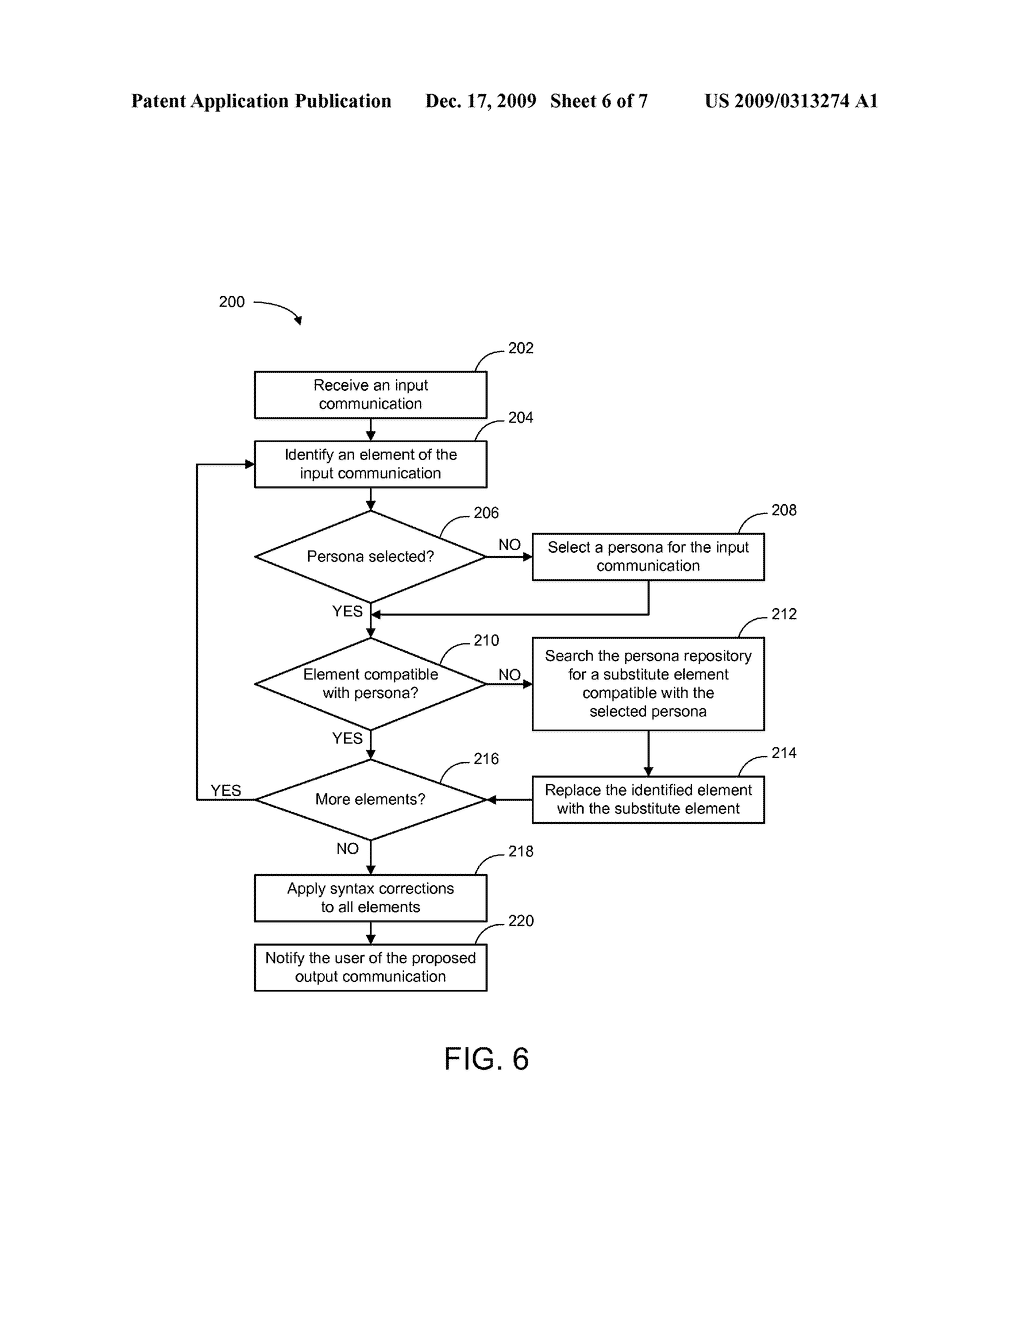
\includegraphics[width=0.7\linewidth]{img/persona_management_flow.png}
    \caption{Persona Management}
    \label{fig:persona_management_workflow}
\end{figure}



% \subsection{MapReduce}
MapReduce is a programming framework designed to simply processing data on large clusters \cite{mapreduce}. MapReduce works by the user supplying two functions, Map and Reduce, which operate in parallel on the data set provided. The Map function processes data from key/value pairs into an intermediate set of key/value pairs, before the Reduce function processes this intermediate set into final key/value pairs.

\lstset{language=C++,caption={Calculating the frequency of words in files using MapReduce \cite{mapreduce}},label=lst:mapreduceexample,tabsize=2,breaklines=true,breakatwhitespace=true,frame=single}
\begin{lstlisting}[float]
map(String key, String value):
	// key: document name
	// value: document contents
	for each word w in value:
		EmitIntermediate(w, ``1'');
		
reduce(String key, Iterator values):
	// key: a word
	// values: a list of counts
	int result = 0;
	for each v in values:
		result += ParseInt(v);
	Emit(AsString(result));	
\end{lstlisting}

Listing \ref{lst:mapreduceexample} is an example MapReduce program which counts the frequency of words within a selection of documents stored on a system. The Map function reads each word, \emph{w}, and emits the word as key/value pair \verb/(w, ``1'')/ to signify that there is an occurrence of \emph{w} at that position. The Reduce function sums together the value each of these emitted key/value pairs, where the key is the same, and emits the sum for each word.

Whilst the example given in Listing \ref{lst:mapreduceexample} uses Strings for the input and output for both of the Map and Reduce functions, it is not necessarily the case that all Map and Reduce functions operate in this way. \cite{mapreduce} explains that the types used by both are linked, as shown by:

\begin{verbatim}
map     (k1, v1)        -> list(k2, v2)
reduce  (k2, list(v2))  -> list(v2)
\end{verbatim}

This states the input keys and values are from a different domain to the output keys and values, which also means that the types used can differ.

MapReduce operates in two phases: The Map phase and the Reduce phase. Initially, the input data is split into small chunks to be assigned to the map tasks. A single map task is designated the master, with the remaining tasks designated as workers. The master assigns each map task a chunk of the input data to process, and once this has been processed, it is assigned more until all the input data has been processed. Once data from a map task has been processed, available reduce tasks then process this into the output data from the MapReduce program.

The MapReduce framework is highly fault tolerant, and is able to cope with multiple worker failure and failure of the master program as well. Each worker is required to periodically communicate with the master, and if no communication is received, then the worker is marked as failed, and its work is redistributed back out to be processed again. In case of the master failing, checkpoints are made and the MapReduce program can restart from the last checkpoint recorded.

\subsubsection{Google File System}
The Google File System, GFS, provides the distributed file system which MapReduce operates with \cite{mapreduce}, but was developed outside of MapReduce to address issues found with previous distributed file systems \cite{gfs}.

The GFS was designed to meet three major points identified with existing distributed file systems \cite{gfs}:
\begin{enumerate}
	\item Component failures are the norm, rather than the exception
	\item Files are huge by traditional standards
	\item Files are mutated by appending new data
\end{enumerate}

As hardware failures are common, the design of the GFS incorporates this, and the system is monitoring itself continually to detect, tolerate, and recover promptly from component failures on a routine basis \cite{gfs}. In addition to this, the system used by Google makes use of inexpensive hardware due to the frequent failures experienced, and as such is a more cost-effective solution than using more expensive tailored hardware.

A GFS cluster is split into a single $master$ and multiple $chunkservers$ and is accessed by multiple $clients$ \cite{gfs}. Files stored in the GFS are split into chunks, which are stored across the cluster on the hard disks located on each chunkserver. By default, each chunk is replicated in the file system three times for reliability of access to data within file system.

Files are stored into the GFS in chunks of size 64MB. This size was chosen to reduce the need to interact with master to find the location of chunks to read data from, and write data to. The larger chunk size also reduces the quantity of metadata stored on the master, which increases the performance of the master as the metadata can be stored in memory, reducing lookup times \cite{gfs}.

The master node maintains the metadata for the file system. This includes the locations of chunks across the file system, and which chunks compose the files stored. The master node communicates with each chunkserver frequently, and if it does not receive a response, the chunkserver is deemed to have failed and any chunks which are then under replicated in the file system are re-replicated to ensure that the minimum number of replications for each chunk are observed.

\subsection{Hadoop}
Hadoop\footnote{\url{http://hadoop.apache.org/}} is framework for performing
distributed computing. It is a free implementation of the MapReduce framework
developed at Google, and is also a top-level project hosted by Apache.

Hadoop has diversified itself from its conception, and is now composed of three
subprojects, Hadoop Common, Haddop Distributed File System, and Hadoop
MapReduce. Hadoop Common providse common utilities which support the other
Hadoop subprojects. The Hadoop Distributed File System is described in more
detail in Section \ref{sec:hdfs}

Hadoop MapReduce is the subproject by which Hadoop itself more known for. It
provides functionality similar to the MapReduce framework developed by Google,
where there exists a $Map$ and a $Reduce$ function which process data across a
cluster.

\subsubsection{Hadoop Distributed File System}
\label{sec:hdfs}
Hadoop also provides a the Hadoop Distributed File System, HDFS. The HDFS is a free implementation of the Google File System, and is designed to be used with Hadoop itself, though can also be used a distributed file system by itself \cite{hdfs}.

The HDFS operates in a similar approach to the operation of Hadoop and the Google File System. There exists a master node, called the NameNode, and many slave nodes, called DataNodes. The NameNode co-ordinates the access of files stored in the HDFS, and also manages the file system namespace. There is usually a DataNode present on each physical node within the cluster. It is the DataNode which control the storage of files on the storage system present on the node, and also controls the reading and writing of files to the HDFS from a user.

The HDFS ensures data integrity through replication of data across different nodes within the cluster. A replication factor is set for the cluster, generally at least 3, which causes all data within the HDFS to be replicated at least that many times. Data within the HDFS is split into blocks, with a large file being represented by many smaller blocks, and it is these blocks which are replicated across the HDFS.

In case of a problem with the HDFS, such as a partial network failure, or hard disk failure, each DataNode is required to periodically message the NameNode which contains a report on all data blocks stored by that DataNode. If there is a failure of some kind, then the NameNode either receives an incomplete message or no message at all. This informs the NameNode that there is a problem with the HDFS and takes appropriate action, including re-replicating the lost data from other DataNodes to new DataNodes.

The HDFS also provides another service called the SecondaryNameNode. The SecondaryNameNode is not a direct failover service to the NameNode. Instead, the SecondaryNameNode takes periodic checkpoints of the state of the NameNode, so that in case of the NameNode failing, a recent copy of the state of the HDFS can be loaded when the NameNode is restarted, which should result in minimal problems with resuming the HDFS.

